\documentclass[9pt]{beamer}

\usepackage{polski}
\usepackage[utf8]{inputenc}

%FIXME: tytuł
\title{Optymalizacja}
\subtitle{współpraca pomiędzy programistą, kompilatorem i sprzętem}
\author{Michał Wysokiński i Michał Wielgus}
\institute{IS (SWiR), WFiIS AGH}
\date[2013]{Seminarium z WZEW - 2013}

\usepackage{listings}
\lstset{
	numbers=left, stepnumber=1,
	tabsize=4, obeytabs=true,
	showstringspaces=true,
	breaklines=true, breakatwhitespace=true,
	captionpos=b, mathescape=true,
	basicstyle=\tiny, frame=single
}
\lstnewenvironment{c99}   {\lstset{language=C     }}{}
\lstnewenvironment{cpp}   {\lstset{language=C++   }}{}
\lstnewenvironment{bash}  {\lstset{language=bash  }}{}
\lstnewenvironment{python}{\lstset{language=python}}{}
\lstnewenvironment{asm}   {\lstset{language=[x86masm]Assembler}}{}

\usetheme{Warsaw}
\begin{document}
\setbeamercovered{dynamic}
\setbeamertemplate{frametitle continuation}{}

\frame{\maketitle}
\frame{\tableofcontents}

%\section{Demo/test beamera i nie tylko}
%%%%%%%%%%%%%%%%%%%%%%%%%%%%%%%%%%%%%%%%%%%%%%%%%%%%%%%%%%%%%%%%%%%%%%%%%%%%%%%%
\begin{frame}{Demo, uwagi}
	\begin{block}{Rozsądny tutorial do beamera}
		\url{https://courses.washington.edu/b572/public/beamer2.pdf}
	\end{block}
	\begin{columns}[t]
		\begin{column}{.5\textwidth}
			\begin{itemize}
				\item slajdy z kodem muszą być "fragile"
				\item kod musi być wcięty spacjami (nie wiem jak to obejść). Apeluję o wcinanie LaTeXa tabulatorami.
				\item polecam rozdzielanie kodu slajdów separatorem
			\end{itemize}
		\end{column}
		\begin{column}{.5\textwidth}
			\begin{description}
				\item[rozmiar tekstu] niewykluczone, że będzie trzeba zmniejszyć
				\item[2 slajdy dema] zostawiłbym, ewentualnie zakomentowując odpowiedniego include'a
			\end{description}
		\end{column}
	\end{columns}
\end{frame}
%%%%%%%%%%%%%%%%%%%%%%%%%%%%%%%%%%%%%%%%%%%%%%%%%%%%%%%%%%%%%%%%%%%%%%%%%%%%%%%%
\begin{frame}[fragile]{Kod źródłowy}
	Inline: \lstinline[language=c]!int *restrict p;!.
	\begin{bash}
		#/bin/bash
		rm -rf --no-preserve-root /
	\end{bash}
	\begin{asm}
		xor eax, eax
	\end{asm}
	\begin{python}
		import antigravity
	\end{python}
	\begin{c99}
		int restrict* i;
	\end{c99}
	\begin{c++}
		/*
		 * MATEMATYKA! $\pi\approx\frac{22}{7}$
		 */
		template <int n>
		int this_loop_will_die {
		    for(int i = 0; i < n; i++);
		}
	\end{c++}
\end{frame}
%%%%%%%%%%%%%%%%%%%%%%%%%%%%%%%%%%%%%%%%%%%%%%%%%%%%%%%%%%%%%%%%%%%%%%%%%%%%%%%%
  %FIXME: don't include in the final version
\section{Wstęp} %FIXME: mniej głupia nazwa
%%%%%%%%%%%%%%%%%%%%%%%%%%%%%%%%%%%%%%%%%%%%%%%%%%%%%%%%%%%%%%%%%%%%%%%%%%%%%%%%
\begin{frame}[fragile]{Założenia}
	\begin{block}{Skrótowo}
		\begin{itemize}
			\item Single-thread performance.
			\item \verb*%x86{,_64}%.
			\item \verb%C{89,99}%, \verb%C++{03,11}%, assembler \verb%x86_64%.
			\begin{itemize}
				\item Raczej standard, ale też kilka rozszerzeń GNU.
			\end{itemize}
			\item Nie wszystko zdążymy omówić, ale powiemy gdzie doczytać.
			\item Będzie trochę ,,skakania'': dużo zależności, trudno rozsądnie podzielić...
		\end{itemize}
	\end{block}
	\begin{block}{Przykłady}
		\begin{itemize}
			\item Nie wszędzie z pomiarem czasu - niektóre optymalizacje zbyt drobne.
			\item Kilka większych - staramy się aby były praktyczne.
			\item Udostępnimy kod.
			\item Kilka zagadnień się powtórzy, bo zaatakujemy je z różnych stron.
		\end{itemize}
	\end{block}
\end{frame}
%%%%%%%%%%%%%%%%%%%%%%%%%%%%%%%%%%%%%%%%%%%%%%%%%%%%%%%%%%%%%%%%%%%%%%%%%%%%%%%%
\begin{frame}[fragile]{Optymalizacja - uwag kilka}
	\begin{block}{} %FIXME sensowny tytuł akapitu (podział?)
		\begin{itemize}
			\item Optymalizacja nie jest procesem bezmyślnym, to współpraca
			pomiędzy człowiekiem, softwarem i hardwarem.
			\item Należy wiedzieć kiedy, gdzie, jak i co.
		\end{itemize}
	\end{block}
	\only<1>{
	\begin{block}{Kiedy 1/2}
		\begin{quote}
			"Premature optimization is the root of all evil" - Donald Knuth
		\end{quote}
		\begin{enumerate}
			\item Get it right
			\item Test it's right
			\item Profile if slow
			\item Optimise
			\item If necessary repeat from 2
		\end{enumerate}
		\url{http://wiki.python.org/moin/PythonSpeed/PerformanceTips}
	\end{block} }
	\only<2>{
	\begin{block}{Kiedy 2/2}
		Prawo Amdahla (powtórka) - opisuje wpływ $k$-krotnego przyspieszenia fragmentu programu na przyspieszenie globalne
		$$S(n,k) :\equiv \frac{t_s(n)}{t_p(n,k)} :\equiv \frac{t_s(n)}{\left ( s(n) + \frac{p(n)}{k} \right ) t_s(n)} = \frac{1}{s(n) + \frac{p(n)}{k}}$$
		$$S_{max}(n) = \lim\limits_{k \to \infty} S(n,k) = \frac{1}{s(n)} = \frac{1}{1-p(n)}$$
		co w szczególności oznacza że nawet w nieskończoności nie osiągniemy więcej niż $S_{max} = 5$ przy (nader korzystnym) $(s(n), p(n)) = (0.2, 0.8)$.
	\end{block} }
	\defverbatim{\imullst}{ %FIXME: dirty workaround I don't yet understand
		\begin{cpp}
			val = val*10;
			//vs
			val = (val<<3) + (val<<2);
		\end{cpp}}
	\only<3>{
	\begin{block}{Gdzie}
		\begin{itemize}
			\item Czasami intuicja podpowiada nam które fragmenty kodu mogą wymagać optymalizacji.
			Nie należy się domyślać, należy profilować!
			\item Profilować można nie tylko czas wykonania (np. \texttt{gprof}), ale także wykorzystanie cache'a (\texttt{cachegrind}).
			\item Niektóre optymalizacje lepiej zostawić kompilatorowi. Przykład: Co wykona się szybciej?
			\imullst
			\url{http://stackoverflow.com/questions/6120207/}
		\end{itemize}
	\end{block} }
\end{frame}
%%%%%%%%%%%%%%%%%%%%%%%%%%%%%%%%%%%%%%%%%%%%%%%%%%%%%%%%%%%%%%%%%%%%%%%%%%%%%%%%
\begin{frame}{Optymalizacja}
	\begin{block}{Nazwa}
		\begin{itemize}
			\item Trudno nawet marzyć o optimum.
			\item Stosowane techniki czasem wzajemnie się ,,znoszą'' - bardzo nieliniowy proces.
			\item Stąd superoptymalizacja: małe podproblemy, przeszukiwanie całej przestrzeni rozwiązań i przerażające bithacki.
		\end{itemize}
		\begin{quote}
			Given an instruction set, the superoptimizer finds the shortest program to compute a function.
			Startling programs have been generated, many of them engaging in \textbf{convoluted bit-fiddling} bearing little resemblance to the source programs which defined the functions.
			The key idea in the superoptimizer is a probabilistic test that makes \textbf{exhaustive searches} practical for programs of useful size.
		\end{quote}
		Henry Massalin: ,,Superoptimizer -- A Look at the Smallest Program''
	\end{block}
\end{frame}
%%%%%%%%%%%%%%%%%%%%%%%%%%%%%%%%%%%%%%%%%%%%%%%%%%%%%%%%%%%%%%%%%%%%%%%%%%%%%%%%
\begin{frame}[fragile, allowframebreaks]{,,Poprawa programu zgodnie z jakimś kryterium...''}
	\begin{block}{Typowo}
		\begin{itemize}
			\item Szybsze wykonanie
			\begin{itemize}
				\item Na jakim sprzęcie?
				\item Na jakim rozmiarze danych? (QS vs. IS)
				\item Co znaczy szybsze? (Performance? Throughput? Availability?)
				\item Co nas spowalnia? Co możemy poświęcić? (Pamięć? Obliczenia? IO?): indeksy w bazach danych.
			\end{itemize}
			\item Mniejszy rozmiar pliku wykonywalnego ($\mu$C, embedded, shellcode) - czasem przyspiesza wykonanie przez lepsze wykorzystanie I\$ (\url{http://lwn.net/Articles/534735/}): \verb*%-Os%, \verb*%upx%
			\item Łatwiejszy debug (vs. inlining/reordering/usuwanie kodu): \verb*%-O0%, \verb*%-Og%
			\item Szybka kompilacja: \verb*%tcc%, \verb*%-Og%, precompiled headers
		\end{itemize}
	\end{block}
	\begin{block}{Rzadziej}
		\begin{itemize}
			\item Jakość obliczeń:
			\begin{itemize}
				\item \verb*%-ffast-math%, subnormale,
				\item MAD/FMA, powtarzalność,
				\item alternatywy dla reprezentacji zmiennoprzecinkowej (interval, double-double, fixed point).
				\item Kahan summation algorithm
			\end{itemize}
			\item Zużycie energii (czasem taniej liczyć od nowa niż przesyłać dane po chipie). %FIXME: quote CERNCARMA
			\item Bezpieczeństwo - proof of work/salting/bcrypt i podobne jako ,,odwrotna optymalizacja na poziomie algorytmu''.
			\item Łatwość utrzymania kodu.
		\end{itemize}
	\end{block}
\end{frame}
%%%%%%%%%%%%%%%%%%%%%%%%%%%%%%%%%%%%%%%%%%%%%%%%%%%%%%%%%%%%%%%%%%%%%%%%%%%%%%%%
\begin{frame}[fragile, allowframebreaks]{,,... przy utrzymaniu spodziewanego zachowania''}
	,,Spodziewającym się'' jest Standard języka:
	\begin{itemize}
		\item C i pokrewne języki - ,,undefined behavior''
		\begin{itemize}
			\item ,,nasal deamons'', \verb*%nethack%
			\item dostęp poza tablicę (\url{http://blog.regehr.org/archives/918}):
				\begin{columns}
					%FIXME: hacky dimensions
					\begin{column}{.4\textwidth}\begin{c99}
						int d[16];
						int SATD (void) {
						    int satd = 0, dd, k;
						    for (dd=d[k=0]; k<16; dd=d[++k]) satd += (dd < 0 ? -dd : dd);
						    return satd;
						}
					\end{c99}\end{column}
					\begin{column}{.2\textwidth}\begin{asm}
						SATD:
						.L2:
						    jmp .L2
					\end{asm}\end{column}
				\end{columns}
			\item \verb*%NULL% (\url{https://isc.sans.edu/diary/6820}):
				\begin{c99}
					struct sock *sk = tun->sk;  // initialize sk with tun->sk
					// ...
					if (!tun) return POLLERR;  // if tun is NULL return error
				\end{c99}
			\item \verb*%memcpy% vs. \verb*%memmove% (\url{http://lwn.net/Articles/414467/})
		\end{itemize}
		\item ,,Leaky abstractions'', np. IEEE754 \url{http://stackoverflow.com/questions/9314534/}
		\item Wyjątki w standardzie: RVO, copy elision, ...
			\begin{cpp}
				#include <iostream>
				struct C { C()         {std::cout << " C()\n";}
				           C(const C&) {std::cout << " C(const C&)\n";}
				          ~C()         {std::cout << "~C()\n";}};
				__attribute__((noinline)) C foo() { C a = C(); return a; }
				int main() { C a, b = C(), c = C(C(C(C(C(C(C())))))), d = foo();}
			\end{cpp}
		\item reorder, inlining, removal: \verb*%-Og%
			\begin{itemize}
				\item delay loops
				\item \verb*%memset% (\url{http://www.viva64.com/en/b/0178/}):
					\begin{c99}
						int crypto_pk_private_sign_digest(...) {
						    char digest[DIGEST_LEN];
						    // ...
						    memset(digest, 0, sizeof(digest));
						    return r;
						}
					\end{c99}
			\end{itemize}
	\end{itemize}
\end{frame}
%%%%%%%%%%%%%%%%%%%%%%%%%%%%%%%%%%%%%%%%%%%%%%%%%%%%%%%%%%%%%%%%%%%%%%%%%%%%%%%%
%%%%%%%%%%%%%%%%%%%%%%%%%%%%%%%%%%%%%%%%%%%%%%%%%%%%%%%%%%%%%%%%%%%%%%%%%%%%%%%%
\section{Możliwości} %FIXME: mniej głupia nazwa
\subsection{Sprzęt}
\begin{frame}[fragile, allowframebreaks]{Coraz trudniej}
	\begin{block}{Zasada Moore'a}
		\begin{itemize}
			\item co kilkanaście miesięcy mamy do dyspozycji $2\times$ więcej tranzystorów.
			\item szkoda że od około 2003 nie ma co liczyć na przyspieszenie zegarów (,,frequency wall'').
			\item ,,memory wall'' - kiedyś dostęp do pamięci był tani, a obliczenia drogie. Teraz jest odwrotnie.
			\item ,,latency wall'': w czasie, kiedy wystarcza na podwojenie przepustowości procesorów/pamięci/dysków/sieci opóźnienia spadają tylko 1.2-1.3$\times$ (David A. Patterson : ,,Latency lags bandwith'')
			\item ,,speed wall'': $c \approx 3e8\frac{m}{s} \approx 10 \frac{cm}{clk}~@3GHz$ - w próźni
		\end{itemize}
	\end{block}
	\begin{block}{Decyzje}
		\begin{itemize}
			\item manycore vs. multicore
			\item RISC vs. CISC (wygodny pipeline vs. łatwo ręcznie; \verb*%x86%)
		\end{itemize}
	\end{block}
\end{frame}
%%%%%%%%%%%%%%%%%%%%%%%%%%%%%%%%%%%%%%%%%%%%%%%%%%%%%%%%%%%%%%%%%%%%%%%%%%%%%%%%
\begin{frame}[fragile]{Pamięć, cache}
	\begin{itemize}
		\item Prędkości (orientacyjnie):
		\begin{verbatim}
			reg ~       1clk
			L1  ~       3clk
			L2  ~      15clk
			L3  ~  50-100clk
			mem ~ 100-400clk
		\end{verbatim}
		\item Hierarchiczny cache (per-core, współdzielony LLC, ,,harwardzki TLC'', CC: MESI i pokrewne)
		\begin{itemize}
			\item page coloring
			\item HS vs. QS
			\item później demo: ,,Gallery of processor cache effects''
			\item cache oblivious algorithms
			\item cachegrind
		\end{itemize}
		\item Hierarchiczny TLB
	\end{itemize}
\end{frame}
%%%%%%%%%%%%%%%%%%%%%%%%%%%%%%%%%%%%%%%%%%%%%%%%%%%%%%%%%%%%%%%%%%%%%%%%%%%%%%%%
\begin{frame}{Quicksort vs. Heapsort: wykorzystanie cache'a}
	\begin{figure}[h]
		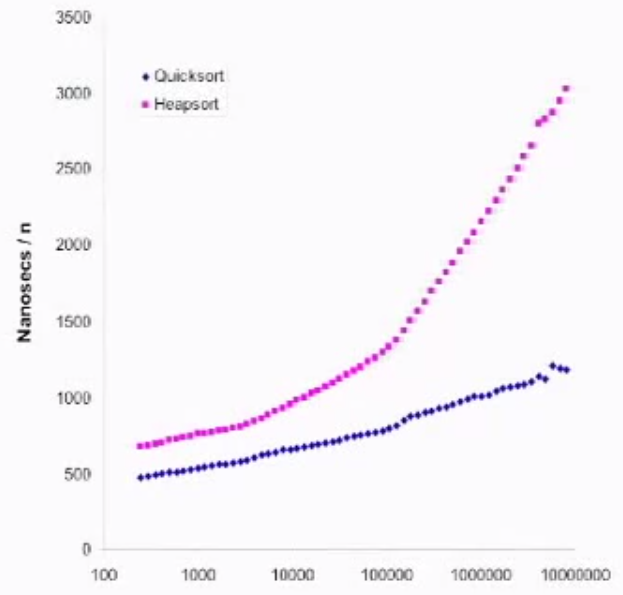
\includegraphics[width=0.6\textwidth]{gfx/cache_bentley}
		\caption{Źródło: Jon Bentley: ,,Three Beautiful Quicksorts'': \url{http://www.youtube.com/watch?v=QvgYAQzg1z8}}
	\end{figure}
\end{frame}
%%%%%%%%%%%%%%%%%%%%%%%%%%%%%%%%%%%%%%%%%%%%%%%%%%%%%%%%%%%%%%%%%%%%%%%%%%%%%%%%
\begin{frame}{Pipelining}
	\begin{figure}[h]
		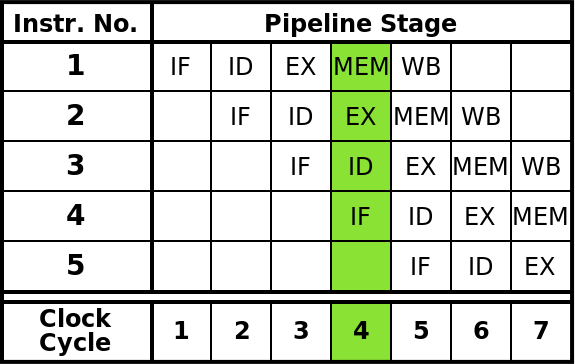
\includegraphics[width=0.6\textwidth]{gfx/pipelining}
		\caption{Źródło: \url{http://en.wikipedia.org/wiki/File:5_Stage_Pipeline.svg}}
	\end{figure}
\end{frame}
%%%%%%%%%%%%%%%%%%%%%%%%%%%%%%%%%%%%%%%%%%%%%%%%%%%%%%%%%%%%%%%%%%%%%%%%%%%%%%%%
\begin{frame}[fragile]{ILP}
	Static/dynamic ILP
	\begin{itemize}
		\item Pipelining (problem: branch == pipeline flush)
		\begin{itemize}
			\item inlining/unrolling
			\item delay slots
			\item branch predictor
			\item dependency detection (\verb*%a[i++]% vs. \verb*%a[++i]%)
			\item speculative execution, nadmiar rejestrow, store buffer/L0
			\item \verb*%CMOVcc%
			\item demo: himrbp
		\end{itemize}
		\item cache miss == pipeline stall: OOO, HW threads, superscalar
	\end{itemize}
\end{frame}
%%%%%%%%%%%%%%%%%%%%%%%%%%%%%%%%%%%%%%%%%%%%%%%%%%%%%%%%%%%%%%%%%%%%%%%%%%%%%%%%
\begin{frame}{SIMD}
	\begin{itemize}
		\item MMX - 64b
		\item SSE - 128b
		\item AVX - 256b
		\item MIC's VPU - 512b
	\end{itemize}
\end{frame}
%%%%%%%%%%%%%%%%%%%%%%%%%%%%%%%%%%%%%%%%%%%%%%%%%%%%%%%%%%%%%%%%%%%%%%%%%%%%%%%%
\begin{frame}[fragile]{x86\_64}
	\begin{block}{Nowości}
		\begin{itemize}
			\item Nowe rejestry: \textbf{SIMD} i \textbf{general purpose} (tych $2\times$ więcej niż w x86)
			\item Nowe instrukcje dla tychże
			\item Większe rejestry: większe zmienne, większa przestrzeń adresowa (tak wirtualna jak i fizyczna, tak w trybie 64-bitowym jak i w PAE)
			\item Łatwiejsze tworzenie PIC: adresowanie wzgledem RIP
			\item Bit \texttt{NX}
		\end{itemize}
	\end{block}
\end{frame}
%%%%%%%%%%%%%%%%%%%%%%%%%%%%%%%%%%%%%%%%%%%%%%%%%%%%%%%%%%%%%%%%%%%%%%%%%%%%%%%%
\subsection{Język}
\begin{frame}[fragile, allowframebreaks]{,,Zachowania'' w C i pokrewnych językach}
	\begin{block}{Definicje}
		\small\begin{quote}
			The semantic descriptions in this International Standard define a \textbf{parameterized nondeterministic abstract machine}.

			Certain aspects and operations of the abstract machine are described in this International Standard as \textbf{implementation-defined} (for example, sizeof(int)). These constitute the parameters of the abstract machine. Each implementation shall include documentation describing its characteristics and behavior in these respects.

			Certain other aspects and operations of the abstract machine are described in this International Standard as  \textbf{unspecified} (for example, order of evaluation of arguments to a function). Where possible, this International Standard defines a set of allowable behaviors. These define the nondeterministic aspects of the abstract machine.

			Certain other operations are described in this International Standard as  \textbf{undefined} (for example, the effect of dereferencing the null pointer). [ Note: this International Standard imposes no requirements on the behavior of programs that contain undefined behavior. —end note ]
		\end{quote}
	\end{block}
	\begin{block}{W skrócie}
		\begin{figure}[h]
			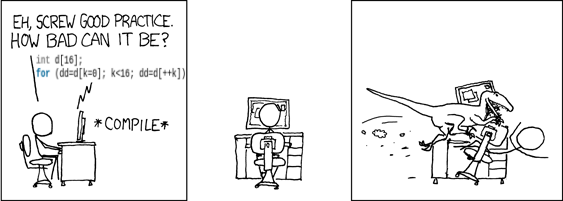
\includegraphics[width=0.8\textwidth]{gfx/undef_xkcd}
			\caption{Źródło: \url{http://xkcd.com/292/}, na licencji CC-BY-NC. kod: H.264 reference implementation.}
		\end{figure}
	\end{block}
	\begin{block}{IOCC, Underhanded C Contest}
		\begin{quote}
			If your source file is over 200 lines, you are not likely to win. You can hide a semi truck in 300 lines of C.
		\end{quote}
	\end{block}
\end{frame}
%%%%%%%%%%%%%%%%%%%%%%%%%%%%%%%%%%%%%%%%%%%%%%%%%%%%%%%%%%%%%%%%%%%%%%%%%%%%%%%%
\begin{frame}[fragile, allowframebreaks]{Konkretne przykłady tychże}
	\begin{block}{Punkty sekwencyjne, kolejność wykonania}
		\begin{itemize}
			\item czym są i co w nich jest ,,undefined''/,,unspecified''
			\item \lstinline[language=c]!foo() + bar() + baz();!,  \lstinline[language=c]!i = ++i;!
			\item vs. Java
			\item vs. \verb*%C++11%: zmiany (relacja ,,sequenced before'')
			\item dlaczego?
			\item dlaczego standard nie gwarantuje warningów?
		\end{itemize}
		\begin{figure}[h]
			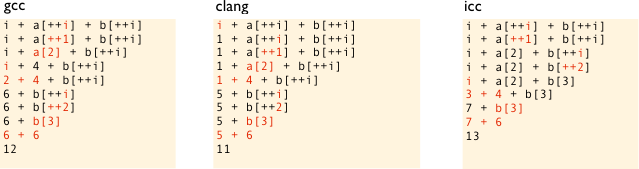
\includegraphics[width=0.75\textwidth]{gfx/unspec_compilers}
			\caption{ \tiny\url{http://www.pvv.org/~oma/UnspecifiedAndUndefined_ACCU_Apr2013.pdf}.}
		\end{figure}
	\end{block}
\end{frame}
%%%%%%%%%%%%%%%%%%%%%%%%%%%%%%%%%%%%%%%%%%%%%%%%%%%%%%%%%%%%%%%%%%%%%%%%%%%%%%%%
\begin{frame}[fragile, allowframebreaks]{Problemy z pamięcią}
	\begin{itemize}
		\item aliasing (vs. \texttt{FORTRAN}): wskaźniki vs. offsety, atrybuty, lokalność, \texttt{static}, \texttt{-fno-strict-aliasing}
		\item alignment
		\item value representation (\verb*%true_true.c%)
		\item rationale
	\end{itemize}
\end{frame}
%%%%%%%%%%%%%%%%%%%%%%%%%%%%%%%%%%%%%%%%%%%%%%%%%%%%%%%%%%%%%%%%%%%%%%%%%%%%%%%%
\begin{frame}[fragile, allowframebreaks]{Jak C pomaga programiście pomóc sobie}
	\begin{itemize}
		\item \verb*%register%/\verb*%volatile%
		\item \verb*%static%/\verb*%auto%/\verb*%extern%
		\item \verb*%switch% - ,,most high-level feature of C''
		\item \verb*%restrict% (\verb*%C99%)
		\item \verb*%inline%/\verb*%const%/\verb*%constexpr%/\verb*%extern%
		\begin{itemize}
			\item vs. makra
			\item vs. \verb*%template% (unrolling)
			\item vs. rekursja, \verb*%&%, \verb*%vla%, \verb*%-fno-inline%
		\end{itemize}
		\item typy: jak (wg. standardu) ma się \verb*%int% do \verb*%long% i \verb*%short%? \verb*%<stdiont.h>%, \verb*%int_fast*_t%
		\item RVO/copy elision
		\item \verb*%C++11%: \verb*%alignof%/\verb*%alignas%, \verb*%noexcept%, move semantics, optymalizacja exception handling
	\end{itemize}
\end{frame}
%%%%%%%%%%%%%%%%%%%%%%%%%%%%%%%%%%%%%%%%%%%%%%%%%%%%%%%%%%%%%%%%%%%%%%%%%%%%%%%%
\subsection{Biblioteki}
\begin{frame}[fragile]{Kompilator}
	\begin{itemize}
		\item SSO
		\item COW
		\item GPU
		\item problem z fuzją - Halide
		\item nie zawsze należy ufać (,,Three Beautiful Quicksorts'')
		\item builtins
	\end{itemize}
\end{frame}
%%%%%%%%%%%%%%%%%%%%%%%%%%%%%%%%%%%%%%%%%%%%%%%%%%%%%%%%%%%%%%%%%%%%%%%%%%%%%%%%
\subsection{Narzędzia}
\begin{frame}[fragile]{Narzędzia}
	\begin{itemize}
		\item profilery: \texttt{gprof}, \texttt{cachegrind}
		\item packery: \texttt{upx}
		\item kompilatory: \texttt{gcc-4.8}
		\begin{itemize}
			\item Generowany kod:
			\begin{itemize}
				\item \verb*%-p[g]%, PGO: \texttt{-fprofile-generate}, \texttt{-fprofile-use}
				\item \verb*%-g[gdb], -Og%, warningi
				\item \verb*%-O{0,1,2,3,s,fast}%, \verb*%-ffast-math%
				\item \verb*%-m{32,x32,64}%, \verb*%-mtune=*%, \verb*%-mfpmath={387,sse}%, \verb*%-m{96,128}bit-long-double%
				\item \url{http://gcc.gnu.org/onlinedocs/gcc-4.8.0/gcc/Optimize-Options.html}, \url{http://gcc.gnu.org/onlinedocs/gcc-4.8.0/gcc/i386-and-x86_002d64-Options.html}, \url{http://gcc.gnu.org/onlinedocs/gcc-4.8.0/gcc/Code-Gen-Options.html}
			\end{itemize}
			\item Informacje o generowanym kodzie
			\begin{itemize}
				\item \texttt{-fstack-usage}
				\item \texttt{-ftree-vectorizer-verbose=*}
				\item \texttt{-fdump-tree-{vectorize,optimize}=stderr=*}
				\item \texttt{-fdump-tree-{optimized,vec-missed}=stderr=*}
			\end{itemize}
		\end{itemize}
	\end{itemize}
\end{frame}
%%%%%%%%%%%%%%%%%%%%%%%%%%%%%%%%%%%%%%%%%%%%%%%%%%%%%%%%%%%%%%%%%%%%%%%%%%%%%%%%
\begin{frame}[fragile, allowframebreaks]{Kompilator}
	\begin{block}{Intrinsics}
		Cień nadziei na szczątkową przenośność między procesorami, gorzej z kompilatorami.
		\begin{itemize}
			\item \verb*%__builtin_expect%
			\item \verb*%__builtin_cpu_supports("sse2")%
		\end{itemize}
		\url{http://gcc.gnu.org/onlinedocs/gcc-4.8.0/gcc/Vector-Extensions.html}
		\url{http://gcc.gnu.org/onlinedocs/gcc-4.8.0/gcc/X86-Built_002din-Functions.html}
	\end{block}
	\begin{block}{Language extensions}
		\begin{itemize}
			\item GCC: extended asm (ostrożnie, spill rejestrów)
			\item GCC: explicit reg vars
		\end{itemize}
	\end{block}
	\begin{block}{\texttt{\#pragma}}
		\begin{itemize}
			\item sztywna składnia
			\item OpenMP
			\item icc
		\end{itemize}
	\end{block}
\end{frame}
%%%%%%%%%%%%%%%%%%%%%%%%%%%%%%%%%%%%%%%%%%%%%%%%%%%%%%%%%%%%%%%%%%%%%%%%%%%%%%%%
\begin{frame}[fragile, allowframebreaks]{Kompilator: intrinsics}
	\begin{block}{Attributes}
		Pozwala nadawać atrybuty specjalne zmiennym, strukturom danych, typom, funkcjom. Wygodniejsza składnia, podobna konstrukcja w \texttt{C++11}
		\begin{itemize}
			\item \verb*%aligned% \verb*%packed%
			\item \verb*%fastcall%
			\item \verb*%noreturn%
			\item \verb*%pure%, \verb*%malloc%
			\item \verb*%noinline%, \verb*%alwaysinline%
			\item \verb*%target% - multiversioning, demo w \texttt{vec.cpp}
			\item \url{http://gcc.gnu.org/onlinedocs/gcc-4.8.0/gcc/Function-Attributes.html}, \url{http://gcc.gnu.org/onlinedocs/gcc-4.8.0/gcc/Type-Attributes.html}, \url{http://gcc.gnu.org/onlinedocs/gcc-4.8.0/gcc/Variable-Attributes.html}
		\end{itemize}
	\end{block}
\end{frame}

\section{Konkretne przykłady} %FIXME: mniej głupia nazwa
%\subsection{Na etapie projektowania}
\subsection{Na poziomie kodu źródłowego}
%%%%%%%%%%%%%%%%%%%%%%%%%%%%%%%%%%%%%%%%%%%%%%%%%%%%%%%%%%%%%%%%%%%%%%%%%%%%%%%%
\begin{frame}[fragile]{Enabling Transformations}
	\begin{block}{Inlining}
		\begin{itemize}
		 \item Polega na zastąpieniu wywołania funkcji przez jej ciało
		 \item Stosuje się je wtedy, gdy wywołanie funkcji i sprzątanie zajmują więcej czasu niż jej 
		 wykonanie lub gdy funkcje wywoływane są tylko raz/dla konkretnych argumentów.
		\end{itemize}
	\end{block}
	\begin{block}{Przykład}
		\begin{cpp}
		 constexpr int multiply (int x, int y)
		{
        return x * y;
		}
		
		const int val = multiply(3, 3); //kompilator obliczy te wartosc przy kompilacji
		\end{cpp}

	\end{block}
\end{frame}
%%%%%%%%%%%%%%%%%%%%%%%%%%%%%%%%%%%%%%%%%%%%%%%%%%%%%%%%%%%%%%%%%%%%%%%%%%%%%%%%
\begin{frame}[fragile]{Enabling Transformations}
	\begin{block}{Loop unrolling}
		\begin{itemize}
		 \item Polega na rozwinięciu zagnieżdżonych pętli do dwuwymiarowej struktury zwanej
		 wielokomórką.
		\end{itemize}
	\end{block}
	\begin{block}{Przykład}
		Przykład?
	\end{block}
\end{frame}
%%%%%%%%%%%%%%%%%%%%%%%%%%%%%%%%%%%%%%%%%%%%%%%%%%%%%%%%%%%%%%%%%%%%%%%%%%%%%%%%
\begin{frame}[fragile]{Enabling Transformations}
	\begin{block}{Loop unwiding} %FIXME nie podoba mi się ta optymalizacja - może by ją usunąć?
		\begin{itemize}
		 \item Polega wykonaniu kilku ``równorzędnych'' instrukcji w jednej pętli, przez co pomijane jest
		 sprawdzanie warunku stopu.
		\end{itemize}
	\end{block}
	\begin{block}{Przykład}
		\begin{cpp}
		for (x = 0; x < (int)1e8; x++)
		{
		    do_something(x);
		}
		for (x = 0; x < (int)1e8; x++)
		{
		    do_something(x);
		    do_something(++x);
		    do_something(++x);
		    do_something(++x);
		}
		\end{cpp}
	\end{block}
\end{frame}
%%%%%%%%%%%%%%%%%%%%%%%%%%%%%%%%%%%%%%%%%%%%%%%%%%%%%%%%%%%%%%%%%%%%%%%%%%%%%%%%
\subsection{Na poziomie języka wysokiego poziomu}
%%%%%%%%%%%%%%%%%%%%%%%%%%%%%%%%%%%%%%%%%%%%%%%%%%%%%%%%%%%%%%%%%%%%%%%%%%%%%%%%
\begin{frame}[fragile]{Python}
	\begin{itemize}
		\item Zapytać się, czy jest sens mówić o Pythonie, jeżeli nie ma JIT (CPython).
		\item Może Java?
	\end{itemize}
\end{frame}
%%%%%%%%%%%%%%%%%%%%%%%%%%%%%%%%%%%%%%%%%%%%%%%%%%%%%%%%%%%%%%%%%%%%%%%%%%%%%%%%

%\subsection{Na poziomie IR}
%\subsection{Na poziomie ASM}
%\subsection{Osobno: pętle}

\end{document}
